\documentclass[border={2pt 5pt 11pt 14pt}]{standalone}
\usepackage{tikz}
\usetikzlibrary{arrows.meta}
\begin{document}
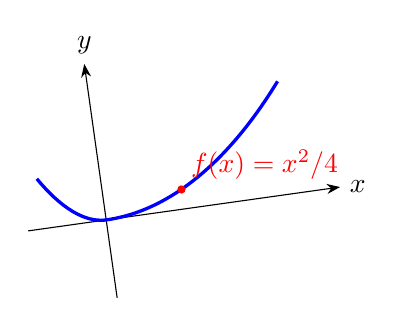
\begin{tikzpicture}[rotate=8]
  \draw[-{Stealth},thin] (-1,0) -- (3,0) node[right] {$x$};
  \draw[-{Stealth},thin] (0,-1) -- (0,2) node[above] {$y$};
  \draw[blue,very thick] (-.8,.64) parabola bend (0,0) (2.4,1.44);
  \fill[red] (1,0.25) circle (1.5pt) node[above right] {$f(x)=x^2/4$};
\end{tikzpicture}
\end{document}
